\PassOptionsToPackage{unicode=true}{hyperref} % options for packages loaded elsewhere
\PassOptionsToPackage{hyphens}{url}
%
\documentclass[]{article}
\usepackage[]{mathpazo}
\usepackage{setspace}
\setstretch{1.25}
\usepackage{amssymb,amsmath}
\usepackage{ifxetex,ifluatex}
\usepackage{fixltx2e} % provides \textsubscript
\ifnum 0\ifxetex 1\fi\ifluatex 1\fi=0 % if pdftex
  \usepackage[T1]{fontenc}
  \usepackage[utf8]{inputenc}
  \usepackage{textcomp} % provides euro and other symbols
\else % if luatex or xelatex
  \usepackage{unicode-math}
  \defaultfontfeatures{Ligatures=TeX,Scale=MatchLowercase}
\fi
% use upquote if available, for straight quotes in verbatim environments
\IfFileExists{upquote.sty}{\usepackage{upquote}}{}
% use microtype if available
\IfFileExists{microtype.sty}{%
\usepackage[]{microtype}
\UseMicrotypeSet[protrusion]{basicmath} % disable protrusion for tt fonts
}{}
\IfFileExists{parskip.sty}{%
\usepackage{parskip}
}{% else
\setlength{\parindent}{0pt}
\setlength{\parskip}{6pt plus 2pt minus 1pt}
}
\usepackage{hyperref}
\hypersetup{
            pdftitle={Improving Deconvolution Methods in Biology through Open Innovation Competitions: an Application to the Connectivity Map},
            pdfauthor={Author 1; Author 2; \ldots{}},
            pdfkeywords={biology, open innoation competitions, crowdsourcing, deconvolution, gene expressions, cell lines},
            pdfborder={0 0 0},
            breaklinks=true}
\urlstyle{same}  % don't use monospace font for urls
\usepackage[margin=1.25in]{geometry}
\usepackage{longtable,booktabs}
% Fix footnotes in tables (requires footnote package)
\IfFileExists{footnote.sty}{\usepackage{footnote}\makesavenoteenv{longtable}}{}
\usepackage{graphicx,grffile}
\makeatletter
\def\maxwidth{\ifdim\Gin@nat@width>\linewidth\linewidth\else\Gin@nat@width\fi}
\def\maxheight{\ifdim\Gin@nat@height>\textheight\textheight\else\Gin@nat@height\fi}
\makeatother
% Scale images if necessary, so that they will not overflow the page
% margins by default, and it is still possible to overwrite the defaults
% using explicit options in \includegraphics[width, height, ...]{}
\setkeys{Gin}{width=\maxwidth,height=\maxheight,keepaspectratio}
\setlength{\emergencystretch}{3em}  % prevent overfull lines
\providecommand{\tightlist}{%
  \setlength{\itemsep}{0pt}\setlength{\parskip}{0pt}}
\setcounter{secnumdepth}{5}
% Redefines (sub)paragraphs to behave more like sections
\ifx\paragraph\undefined\else
\let\oldparagraph\paragraph
\renewcommand{\paragraph}[1]{\oldparagraph{#1}\mbox{}}
\fi
\ifx\subparagraph\undefined\else
\let\oldsubparagraph\subparagraph
\renewcommand{\subparagraph}[1]{\oldsubparagraph{#1}\mbox{}}
\fi

% set default figure placement to htbp
\makeatletter
\def\fps@figure{htbp}
\makeatother

\usepackage{bbm}
\newcommand\hl{}
\newcommand\Fig[1]{{\it Fig. \ref{fig:#1}}}
\usepackage{setspace}
\onehalfspacing

% Custom AB
\usepackage{booktabs}
\usepackage{longtable}
\usepackage{array}
\usepackage{multirow}
\usepackage[table]{xcolor}
\usepackage{wrapfig}
\usepackage{float}
\usepackage{colortbl}
\usepackage{pdflscape}
\usepackage{tabu}
\usepackage{threeparttable}
\usepackage{threeparttablex}
\usepackage[normalem]{ulem}
\usepackage{makecell}
\renewcommand*{\arraystretch}{1.2}


\title{Improving Deconvolution Methods in Biology through Open Innovation
Competitions: an Application to the Connectivity Map}
\author{Author 1 \and Author 2 \and \ldots{}}
\date{Last updated: Sep 05, 2019}

\begin{document}
\maketitle
\begin{abstract}
Report results fo open innovation competition aimed at solving a
gene-related deconvolution problem.


\smallskip\noindent 
Keywords: biology; open innoation competitions; crowdsourcing; deconvolution; gene expressions; cell lines.
\end{abstract}

{
\setcounter{tocdepth}{2}
\newpage
\tableofcontents
\newpage
}
\color{red}

TODOS:

\begin{itemize}
\tightlist
\item
  Check length requirements for Nat. Met.
\item
  Intro {[}AB{]}
\item
  Methdos TN {[}DONE{]}
\item
  Clustering
\item
  Add disaggregated data
\end{itemize}

\color{black}

\hypertarget{introduction}{%
\section{Introduction}\label{introduction}}

Many recent examples have shown significant benefits for drug discovery
from the systematic analysis of large repositories of gene-expression
profiles {[}Refs{]}. However, traditional gene-expression
high-throughput profiling technologies that are based multianalyte
methods, such as Luminex profiling technology, are limited by the type
and number of available analytes {[}Refs{]}. Therefore, the cost of big
data generation in biology remains prohibitive.

Using an assay called L1000, The Connectivity Map (CMap) group at the
Broad Institute has developed a novel approach that matches pairs of
genes to the same Luminex beads to double the count of profiled genes
per bead, thus lowering costs {[}Subramanian 2017{]}. A central
component of this approach is to quantify gene-type frequency of beads,
and then statistically deconvolve and compare gene type-specific average
expression profiles for pairs of mixed gene samples.

This type of deconvolution problems are ubiquitous and have a long
history in biology {[}refs{]}. For example, deconvolution problems arise
when trying to identify cell type--specific gene expression differences
in complex tissues {[}Shen-orr et al., 2010{]}; or in the discovery of
target proteins of small molecules {[}Jung, 2015{]}.

Common approaches are parametric (mixture models) and non-parametric.
CMap's current solution to this problem is an algorithm, called
``D-Peak,'' based on a K-means clustering {[}Refs{]}. This method
automatically partitions a set of gene-expression measurements into
\(k\) clusters, taking the mean of the two largest clusters, assigning
the mean value of the largest cluster to the gene in higher proportion
and the mean value of the second largest cluster to the gene in . This
works well but has several problems as well. {[}List problems.{]}
Including time. The trade-off between accuracy and computation time is
currently unknown.

Alternative methods are well known, such as Gaussian etc. But it would
have required substantial resources to experiment with these alternative
approaches (more than what already done) and to adapt new to our data.
Moreover, impossible an exhaustive search for all available approaches
to try; and the combination of these different approaches.

Instead, we used an open innovation competition as a research tool to
engage a variety of computer scientist, software developers and
bioinformatics in the problem. This approach allows simultaneous
exploration of competing approaches tailored to our problem, at no cost.

\hypertarget{methods}{%
\section{Methods}\label{methods}}

In biomedical research, our focus here, deconvolution problems are
common in multianalyte assay methods. These methods are widely used to
do X, Y and Z. In general terms, multianalyte assay methods are based on
microspheres with different fluorescence decay times. This feature can
be used to do X, Y, and Z. {[}EXPLAIN BRIEFLY CMap PROBLEM{]}. One
problem with existing approaches is that they {[}\ldots{}. {]}

To identify accurate methods we launched an open challenge that allowed
a rapid exploration of different approaches. Key ingredients of there
challenges are: training and testing dataset benchmark solution to
improve

\hypertarget{l1000-experimental-scheme}{%
\subsection{L1000 Experimental Scheme}\label{l1000-experimental-scheme}}

The L1000 assay uses Luminex bead-based fluorescent scanners to detect
gene expression changes resulting from treating cultured human cells
with chemical or genetic perturbations {[}Subramanian 2017{]}.
Experiments are performed in 384-well plate format, where each well
contains an independent sample. The Luminex scanner is able to
distinguish between 500 different bead types, or colors, which CMap uses
to measure the expression levels of 978 landmark genes using two
detection approaches.

In the first detection mode, called \(UNI\), each of the 978 landmark
genes is measured individually on one of the 500 Luminex bead colors. In
order to capture all 978 genes, two detection plates are used, each
measuring 489 landmarks. The two detection plates' worth of data are
then computationally combined to reconstruct the full 978-gene
expression profile for each sample.

By contrast, in the \(DUO\) detection scheme two genes are measured
using the same bead color. Each bead color produces an intensity
histogram which characterizes the expression of the two distinct genes.
In the ideal case, each histogram consists of two peaks each
corresponding to a single gene. The genes are mixed in 2:1 ratio, thus
the areas under the peaks have 2:1 ratio (see Figure 1), which enables
the association of each peak with the specific gene. \textbf{The
practical advantage of the DUO detection mode is that it uses half of
the laboratory reagents as UNI mode, and hence \(DUO\) is and has been
the main detection mode used by CMap.}

After \(DUO\) detection, the expression values of the two genes are
computationally extracted in a process called `peak deconvolution,'
described in the next section.

\hypertarget{statistical-deconvolution-of-gene-specific-expression-profiles.}{%
\subsection{Statistical deconvolution of gene-specific expression
profiles.}\label{statistical-deconvolution-of-gene-specific-expression-profiles.}}

In each sample, assume fluorescent-intensity values \(X_{ij}\) for beads
\(i=1,2,\dots, n\) and analytes \(j=1,2,\dots, J\), and gene-specific
proportions \(w_{ik}\) for beads \(i=1,2,\dots, n\) and genes
\(k=1,2,\dots, K\). Our model of analyte fluourescent intensity is: \[
  X_{ij} = \sum_{k=1}^{K} w_{ik} h_{kj} + e_{ij}. 
\] where \(h_{ik}\) is the gene-expression value for genes
\(k=1,2,\dots, K\) and analytes \(j=1,2,\dots, J\).

For the \(UNI\) detection method, the gene-specific proportions are such
that each analyte has only one gene. Hence, \(w^{\text{uni}}_{ik} = 1\)
when \(j = k\), and it is zero otherwise. This implies that each sample
can detect at most \(J\) different genes under the UNI method.

For the \(DUO\) detection method, the gene-specific proportions are such
that each analyte is paired with two genes in 1:2 ratio. Hence, pick an
element \(g\in G^2\) from the set \(G^2\) of all non-overlapping subsets
of size two of the gene set \(G\). For each pair of genes in \(g\)
associated with an analyte \(j\), we have:
\(w^{\text{duo}}_{i1} = 2/3\), \(w_{i2}=1/3\) and is zero otherwise.

\hypertarget{benchmark-k-means-solution}{%
\subsubsection{Benchmark k-means
solution}\label{benchmark-k-means-solution}}

CMap's current solution to this problem is based on a k-means clustering
algorithm called \(dpeak\) that works as follows:

For each measurement, the dpeak partitions the list of realizations into
\(k>=2\) distinct clusters and identifies two of the clusters whose
ratio of membership is as close as possible to 2:1. The algorithm then
takes the median intensity of each of the two clusters, assigning these
values to the appropriate gene (i.e., matching clusters with more
observations to the gene mixed in higher proportion).

After deconvoluting each sample on a plate, dpeak then uses the
plate-wide distributions to perform adjustments on a per-well basis,
correcting peaks that may have been misassigned (see Appendix).

Known problems with the current approach are that k-means is generally a
biased and inconsistent estimator of the peaks of a bimodal distribution
{[}ref{]}. It also sometimes fails to detect peaks with few observations
or it incorrectly identifies these peaks as extraneous and disregards
them. Another limitation is that it is computationally expensive (the
current Matlab implementation takes about 30 minutes on a 12-core server
to process one set of 384 experiments).

\hypertarget{data-generation-for-contest}{%
\subsection{Data generation for
contest}\label{data-generation-for-contest}}

To generate data for this contest, we profiled six 384-well perturbagen
plates, each containing mutually exclusive sets of compound and shRNA
treatments. Multiple treatment types were used to avoid potentially
over-fitting to any one. The compound and shRNA perturbagen plates were
arbitrarily grouped into pairs, and to avoid any potential `information
leakage' each pair was profiled in a different cell line. The resulting
lysates were amplified by ligation mediated amplification (LMA,
Subramanian 2017). The amplicon was then split and detected in both
\(UNI\) and \(DUO\) detection modes. The three pairs of data were
arbitrarily assigned to training, testing, and holdout categories, where
in each case the \(UNI\) data served as the ground truth. Training data
were made available for all the contestants to develop and validate
their solutions offline. The testing data were used to evaluate
solutions during the contestn and populate the live leaderboard. Holdout
data were used evaluate competitors' final submissions and guard against
over-fitting. Prizes were awareded based on performance on the holdout
dataset.

\begin{longtable}[]{@{}ll@{}}
\caption{Data generated}\tabularnewline
\toprule
Category & Type\tabularnewline
\midrule
\endfirsthead
\toprule
Category & Type\tabularnewline
\midrule
\endhead
training & Compounds\tabularnewline
testing & Compounds\tabularnewline
holdout & Compounds\tabularnewline
training & shRNA\tabularnewline
testing & shRNA\tabularnewline
holdout & shRNA\tabularnewline
\bottomrule
\end{longtable}

\hypertarget{scoring-configuation}{%
\subsection{Scoring configuation}\label{scoring-configuation}}

Contest submissions were scored based on accuracy and speed.

\hypertarget{accuracy}{%
\subsubsection{Accuracy}\label{accuracy}}

\color{red}

TODO: update equations to use Latex \color{black}

Accuracy measures were obtained by comparing the contestant's
predictions, which were derived from \(DUO\) data, to the equivalent
\(UNI\) ground truth data generated from the same samples.

The scoring function combines two measures of accuracy: correlation and
AUC, which are applied to deconvoluted (\(DECONV\)) data and one to
differential expression (\(DE\)) data, respectively (See figure XX).

\(DE\) is derived from DECONV by applying a series of transformations
(parametric scaling, quantile normalization, and robust z-scoring) that
are described in detail in Subramanian et al.~2017{[}ref{]}.The
motivation for scoring \(DE\) data in addition to \(DECONV\) is because
it is at this level where the most bilogically interesting gene
expression changes are observed. Of particular interest is obtaining
significant improvement in the detection of, so called, ``extreme
modulations.'' These are genes that notably up- or down-regulated by
pertubation and hence exhibit an exceedingly high (or low) \(DE\) values
relative to a fixed threshold.

\hypertarget{accuracy-based-on-spearman-correlation}{%
\paragraph{Accuracy based on Spearman
correlation}\label{accuracy-based-on-spearman-correlation}}

The first accuracy component is based on the Spearman rank correlation
between the predicted \(DECONV\) data and the corresponding \(UNI\)
ground truth data.

For a given dataset p, let MDUO, p and MUNI, p denote the matrices of
the estimated gene intensities for G = 976 genes (rows) and S
\textasciitilde{} 384 experiments (columns) under DUO and UNI detection.
Compute the Spearman rank correlation matrix between the rows of MDUO, p
and the rows of MUNI, p; take the median of the diagonal elements of the
resulting matrix (i.e., the values corresponding to the matched
experiments between UNI and DUO) to compute the median correlation per
dataset:

CORp = median(diag(spearman(MDUO, p, MUNI, p))

\hypertarget{accuracy-based-on-auc-of-extreme-modulations}{%
\paragraph{Accuracy based on AUC of extreme
modulations}\label{accuracy-based-on-auc-of-extreme-modulations}}

The second component of the scoring function is based on the Area Under
the receiver operating characteristic Curve (AUC) that uses the
competitor's DE values at various thresholds to predict the UNI's DE
values being higher than 2 (``high'') or lower than -2 (``low'').

For a given bead type a in a given dataset p, let AUCp, c denote the
corresponding area under the curve where c = \{ high \textbar{} low \},
where high means UNIDE, p \textgreater{}= 2, and low means UNIDE, p
\textless{}= -2; then, compute the arithmetic mean of the area under the
curve per class to obtain the corresponding score per dataset:

AUCp = (AUCp, hight + AUCp, low) / 2

\hypertarget{speed}{%
\subsubsection{Speed}\label{speed}}

For a given dataset p, the speed component of the score is computed as
the run time in seconds for deconvoluting the data in both test cases:
Runtimep

Notice that multi-theading is allowed in this match, and thus highly
recommended. Your submission will be tested on multi-core machines
(presumably, 8 cores). The maximum execution time of your solution will
be capped by 30 minutes.

\hypertarget{aggregegated-score}{%
\subsubsection{Aggregegated score}\label{aggregegated-score}}

The accuracy and speed components were integrated into a single
aggregate scores as follow:

SCORE = MAX\_SCORE * (MAX(CORp, 0))2 * AUCp2 * exp(- Tsolution / (3 *
Tbenchmark) ) where Tbenchmark is the deconvolution time required by the
reference DPeak implementation

\hypertarget{results}{%
\section{Results}\label{results}}

\hypertarget{participation}{%
\subsection{Participation}\label{participation}}

The contest attracted 294 participants, who made 820 code submissions,
an averge of 18.2 submissions per participant. The top finishers in the
contest employed a variety of different analysis approaches, including
descision tree regressors (DTR), Gaussian mixture models (GMM),
convolutional neural networks (CNN), and customized versions of k-means,
all with notably improved performance relative to the benchmark. Table
xx lists the top 9 finishers and the languages and algorithms each used.

\begin{longtable}[]{@{}lllll@{}}
\caption{Summary of contestant solutions}\tabularnewline
\toprule
rank & handle & language & method & category\tabularnewline
\midrule
\endfirsthead
\toprule
rank & handle & language & method & category\tabularnewline
\midrule
\endhead
1 & gardn999 & Java & random forest regressor & DTR\tabularnewline
2 & Ardavel & C++ & Gaussian mixture model & GMM\tabularnewline
3 & mkagenius & C++ & modified k-means & k-means\tabularnewline
4 & Ramzes2 & Python/C++ & ConvNet & CNN\tabularnewline
5 & vladaburian & Python/C++ & Gaussian mixture model &
GMM\tabularnewline
6 & balajipro & Python/C++ & modified k-means & k-means\tabularnewline
7 & AliGebily & Python & boosted tree regressor & DTR\tabularnewline
8 & LastEmperor & Python & modified k-means & k-means\tabularnewline
9 & mvaudel & Java & other & other\tabularnewline
\bottomrule
\end{longtable}

Fig. 1. Participation stats (Submission counts)

\hypertarget{overall-accuracy-and-speed.}{%
\subsection{Overall accuracy and
speed.}\label{overall-accuracy-and-speed.}}

Using the holdout dataset, we computed the average AUC (on level-four
data), the average rank correlation (level-two data), as well as the
fraction of knocked-down genes correctly predicted for each of the top
solutions and the benchmark. The benchmark achieved an AUC of xxx and
xxx, a correlation of xxx and xxx for plate 1 and 2, respectively, as
well as it successfully predicted xxx knocked-down genes in plate 2. The
corresponding runtime for the benchmark in each plate was of xxx and xxx
seconds.

{\it Fig. \ref{fig:acc-vs-speed}} shows that all top-nine solutions
improved upon the performance of the benchmark in nearly all measures.
Overall, the average AUC improvement was of 2\% (min = xxx, max =xxxx),
the average correlation improvement was of 3\% (min = xxx, max = xxx)
and the average improvement in correct kd genes predictions was of 3\%
(min = xxx, max =xxx). Given a theoretical maximum improvement of xxx,
xxx, and xxx, for the AUC, correlation and KD metrics, we observe that
competitors achieves larger improvements (relative to the maximum
achievable) in the AUC metric.

Only two submissions (out of nine) a performance that was better in AUC
and correlation but worse than the benchmark on the KD success metric.
These submissions, both based on k-means, ranked sixth and eighth in the
final leaderboard.

Improvement with respect to speed were substantial. The average
improvement was 300\% ranging between 100\% and 500\%. We observe no
accuracy-vs-speed trade-off. The empirical relationship between
improvements in accuracy and improvements in speed is essentially flat.

Further examination based on the underlying methods used by the top
solutions suggests that parametric models, such as mixture models, are
both fast and relatively accurate, although non-parametric models, such
as regression forests and k-means, tend to be more accurate. The fastest
algorithm was indeed based on a parametric model, i.e., gaussian mixture
model, which achieves a good level of accuracy on these data. This
solution ranked second overall and achieved the greatest speed
improvmenet in both plates.

The most accurate algorithm was instead based on a random forest. This
solution ranked first overall and achieved the best performance in both
AUC and correlation measures, as well as it was among the top three
approaches in the KD measure.

We observe no significant difference in performance between the plates,
with all the submissions achieving similar scores in both plates.

\color{red}

Todos:

\begin{itemize}
\tightlist
\item
  In Methods section, explain accuracy as measured in the coontest
  (slide p.~124). And then explain, KD additional test of accuracy
  (slides p.~128). Results are good on both.
\item
  (How far froom the max achievable improvement in accuracy
  (down-sampling uni)?)
\item
  Discrepancy between genes with high/low bead counts.
\end{itemize}

\color{black}

\hypertarget{clustering-submissions.}{%
\subsection{Clustering Submissions.}\label{clustering-submissions.}}

Do methods overlap? Not at a level that we care about.

Figure 3. (A) Clustering by genes (high ovverlap); (B) TS1-2 Seem to be
clustering by method (C) Differences mitigated after standard
normalization procedure

\hypertarget{ensambles.}{%
\subsection{Ensambles.}\label{ensambles.}}

Figure 3. (A) Scatterplot runtime vs accuracy for ensamble (slides
p.~163)

Speed vs accuarcy trade-off. Integration one or multiple methods?

\hypertarget{minors}{%
\subsection{Minors:}\label{minors}}

\begin{itemize}
\tightlist
\item
  signs of ovverfitting (compare traing vs testing)
\end{itemize}

\hypertarget{discussion}{%
\section{Discussion}\label{discussion}}

Summary of the results presented in the methods section.

Discussion generality of the solutions

\begin{itemize}
\tightlist
\item
  Novel? Have any of these solutions previously been applied to
  deconvolution problems?
\item
  Specific to this problem or general to others?
\end{itemize}

Discuss implications of these methods for CMap production

\begin{itemize}
\tightlist
\item
  Preliminary results on past data conversion
\item
  Directions for pipeline integration and generation of future data
\item
  Cost savings
\item
  Implementation strategy and outcomes
\item
  Increase in data processing throughput
\end{itemize}

\hypertarget{figures}{%
\section{Figures}\label{figures}}

\hypertarget{scoring-accuracy}{%
\subsection{Scoring accuracy}\label{scoring-accuracy}}

\begin{figure}
\centering
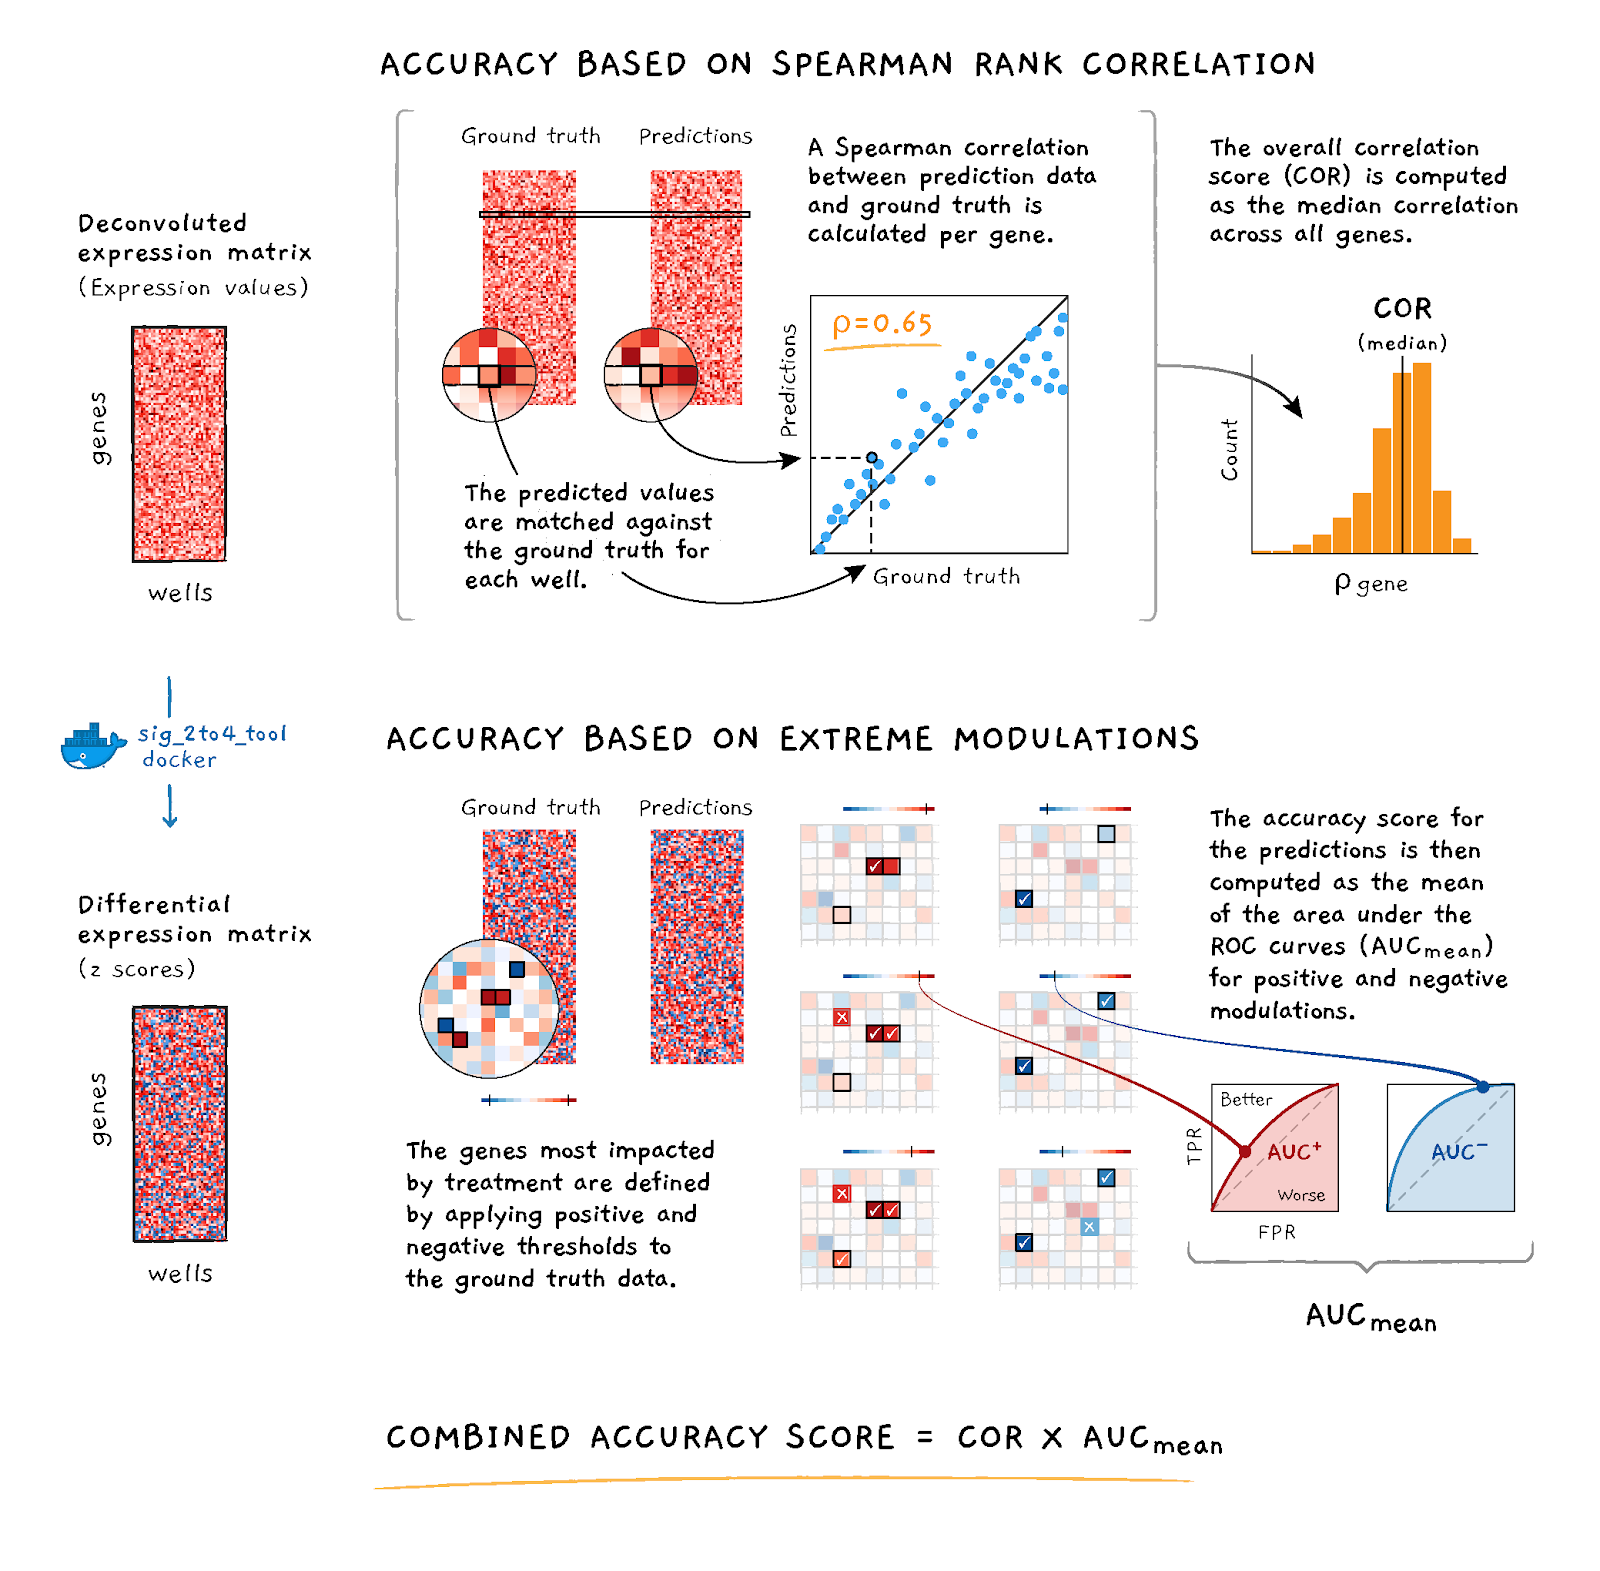
\includegraphics{figures/deconvolution_contest Fig2_Final_revised.png}
\caption{Schematic illustrating accuracy components of scoring function}
\end{figure}

\hypertarget{accuracy-vs.-speed}{%
\subsection{Accuracy vs.~Speed}\label{accuracy-vs.-speed}}

\hypertarget{scoring-accuracy-1}{%
\subsection{Scoring accuracy}\label{scoring-accuracy-1}}

\begin{figure}
\centering
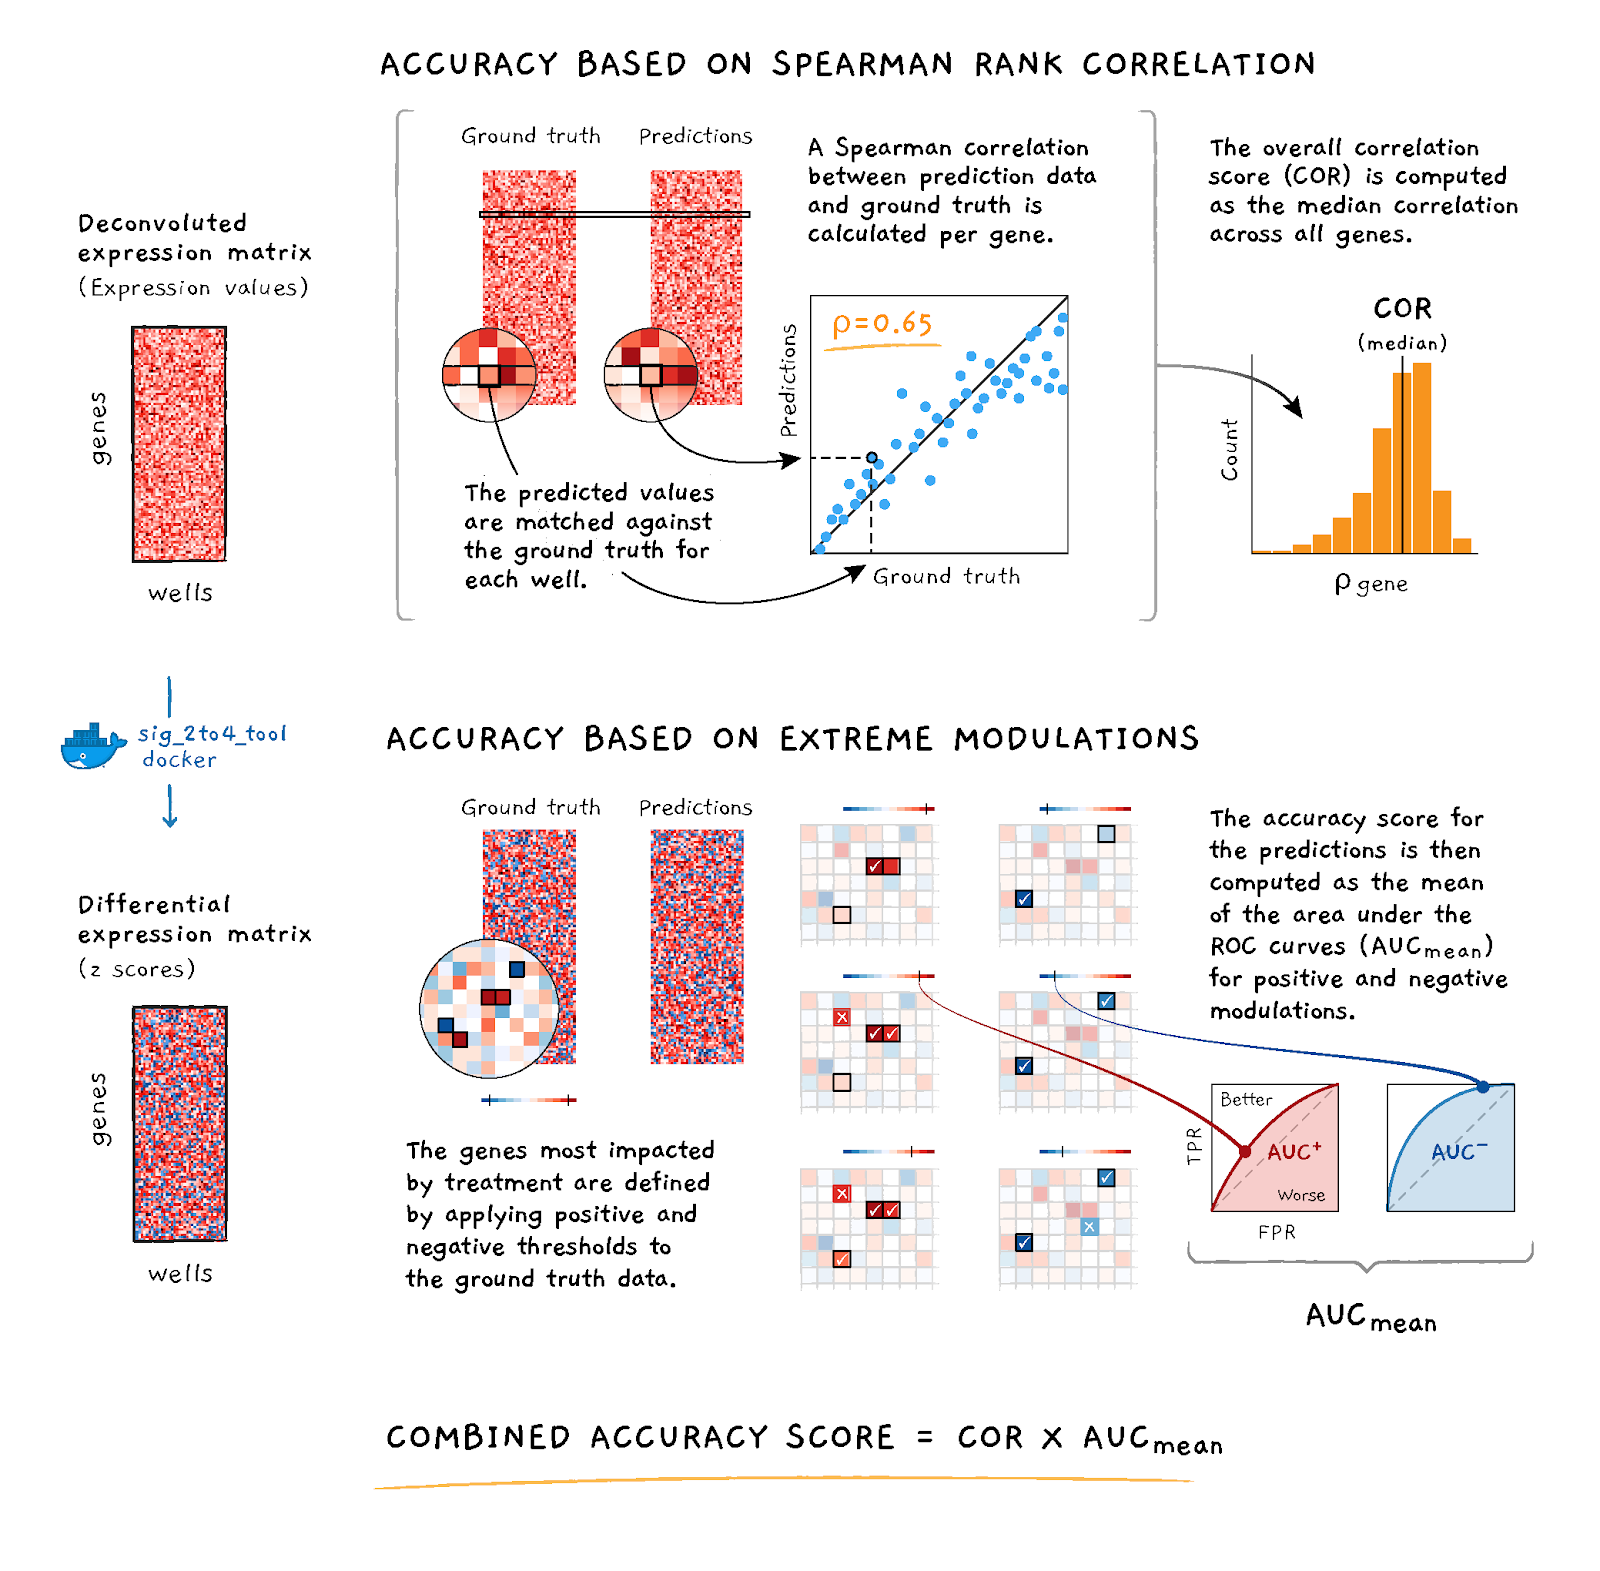
\includegraphics{figures/deconvolution_contest Fig2_Final_revised.png}
\caption{Schematic illustrating accuracy components of scoring function}
\end{figure}

\hypertarget{accuracy-vs.-speed-1}{%
\subsection{Accuracy vs.~Speed}\label{accuracy-vs.-speed-1}}

\begin{figure}
\centering
\includegraphics{main_files/figure-latex/speed_acc-1.pdf}
\caption{\label{speed_acc}Accuracy vs.~Speed}
\end{figure}

\hypertarget{accuracy-vs-speed-ab}{%
\subsection{Accuracy vs speed (AB)}\label{accuracy-vs-speed-ab}}

\begin{figure}
\centering
\includegraphics{main_files/figure-latex/acc-vs-speed-1.pdf}
\caption{\label{fig:acc-vs-speed}\textbf{Accuracy vs speed.} This figure
shows the relationship between improvements in AUC (A.), correlation
(B.) and fraction of correctly predicted knocked-down genes(C.) and
improvements in speed for the top-nine solutions. These measures are
computed for each of the plates on the holdout dataset. Labels at the
dots indicate the rank of the submission in the final leaderboard (1 =
first best, 2 = second best, etc.). Dashed lines indicate levels with no
improvement over the benchmark. Dotted lines indicate (ols) association
between accuracy and speed improvements. The name of the most accurate
and fastest approach are highlighted in each panel.}
\end{figure}

\hypertarget{clustering-of-solutions}{%
\subsection{Clustering of solutions}\label{clustering-of-solutions}}

\begin{figure}
\centering
\includegraphics{main_files/figure-latex/tsne_figure-1.pdf}
\caption{\label{tsne_figure}t-SNE projection of holdout data. Each point
represents the 2D projection of a sample generated by UNI ground truth
(GT) or applying one of the deconvolution algorithms to DUO data. DECONV
data colored by perturbagen type (A) and algorithm type (B). DECONV (C)
and DE (D) data colored by algorithm type and stratified by each
individual implementation.}
\end{figure}

\clearpage

\hypertarget{to-read}{%
\subsection{To read}\label{to-read}}

\begin{itemize}
\tightlist
\item
  \href{https://pubs.rsc.org/en/content/getauthorversionpdf/c4mb00677a}{Compound
  signature detection on LINCS L1000 big data} used a fuzzy c-means
  Gaussian Mixture Model (GMM) to process raw L1000 data, showing better
  performance compared to KNN. This method is described below:
\end{itemize}

\begin{quote}
To deconvolute such overlapped peaks, we assumed that the fluorophore
intensities of each analyte type (corresponding to a specific mRNA type)
had a Gaussian distribution. The distribution of the mixture of analytes
GeneH(i) and GeneL(i) corresponding to the expression levels of GeneH
and GeneL, respectively, should be subject to a bimodal Gaussian
distribution, with the proportion of 1.25 to 0.75. We initialized the
estimations of the two Gaussian distributions using buzzy c-means
clustering {[}11{]} and estimated the GMM parameters using the
Nelder-Mead method {[}12{]}. Thus, the overlapped peaks were
deconvoluted as the two estimated Gaussian peaks and the expression
levels of the two genes sharing the same analyte were extracted.
Mathematical details are included in the Supplementary Methods (the GMM
model).
\end{quote}

\begin{itemize}
\item
  \href{https://ieeexplore.ieee.org/abstract/document/4044778}{Deconvolution
  of linear systems by constrained regression and its relationship to
  the Wiener theory}
\item
  \href{https://www.nature.com/articles/nmeth.2929}{Efficient
  Bayesian-based multiview deconvolution}
\item
  \href{https://www.nature.com/articles/nbt1414}{A Bayesian
  deconvolution strategy for immunoprecipitation-based DNA methylome
  analysis}
\item
  \href{https://www.nature.com/articles/nmeth.1830}{Gene expression
  deconvolution in linear space}
\item
  \href{https://www.nature.com/articles/nmeth.1439}{Cell type--specific
  gene expression differences in complex tissues}
\end{itemize}

\hypertarget{references}{%
\section{References}\label{references}}

\end{document}
